% ==================================================
% CHAPTER 6: Comparing cosmic muon and x-ray relative strip position offsets %
% ==================================================

%TODO : Add the x-ray residual arrow overlay on the cosmics residual TH2. Maybe restructure so all the comparison is in this chapter entirely. 
%TODO : Add this idea in this chapter: "Note that the mean of cosmics residuals around the x-ray points were calculated in bins exactly centered on the nominal x-ray gun position, unlike in figure~\ref{fig:res_mean_th2}."
\chapter{Comparing cosmic muon and x-ray relative strip position offsets}
\label{chap:comparison}
% Edit count: Lia - 1, Brigitte - 0

The goal was to validate the local offsets extracted from the x-ray data with cosmics data. The complication was that the x-ray dataset provided absolute local offsets while the cosmics dataset provided relative local offsets, which could not be compared directly. The solution was to use the x-ray local offsets to calculate a relative local offset. The x-ray relative local offset is the x-ray residual reconstructed from an abstract track using the beam profile centers on each layer as the track hits. The cosmics relative local offset was taken as the Gaussian mean of muon track residuals in a \SI{100}{mm} by \SI{100}{mm} area, referred to the as the mean cosmics residual. Relative local offsets of each type calculated using the same reference layers are compared for each area where x-ray data is available. The  results of the comparison are presented here.

% --------------------------------------------------
% \section{Method for comparing x-ray and cosmics data}
% --------------------------------------------------
%MOVED TO END OF CHAP5, SECTION{MEASURING RELATIVE LOCAL OFFSETS}

%---------------------------------------------------
\section{Assessing correlation}
%---------------------------------------------------
\label{sec:assessing_correlation}
Scatter plots of the x-ray and mean cosmics residuals for two sample quadruplets, referred to as quadruplet 1 and quadruplet 2, in figures~\ref{fig:correlation} and \ref{fig:no_correlation} reveal the degree of correlation between the datasets. 

\begin{figure}
    \centering
    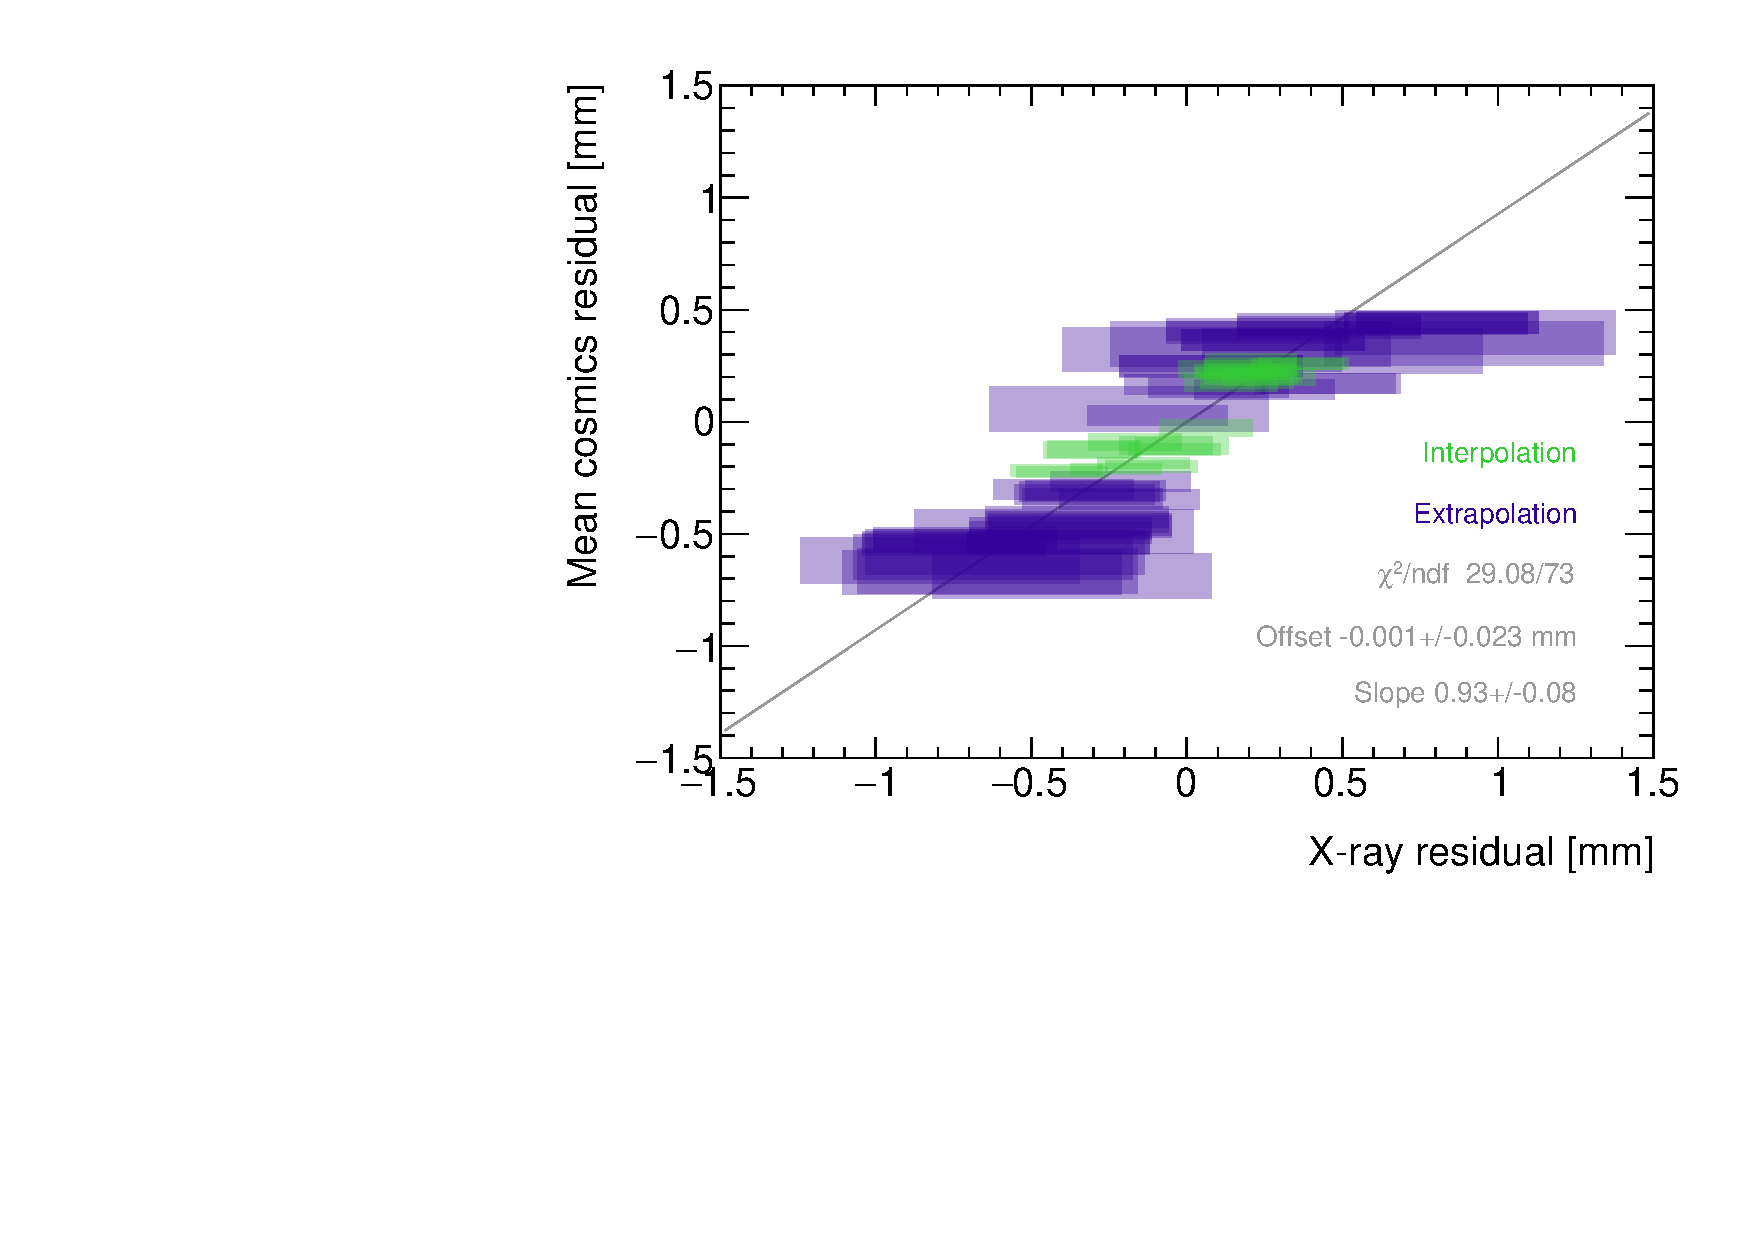
\includegraphics[width = \textwidth]{figures/figure_QL2P11_3100V_2021-08-05_QL2P11_local_cosmic_and_xray_data_correlation_plot.pdf}
    \caption{Correlation plot between x-ray and mean cosmics residuals for all tracking combinations for quadruplet 1. Each rectangle is centered on an x-ray and mean cosmics residual pair calculated at a given gun position and for a certain tracking combination. The width of the rectangles in $x$ and $y$ are the uncertainty in the x-ray and mean cosmics residual respectively. A printer-friendly version of this plot is available in appendix~\ref{appendix:print}.}
    \label{fig:correlation}
\end{figure}

First, the fitted slope and offset in figure~\ref{fig:correlation} show that the two quadruplet 1 datasets are correlated. The magnitude of the uncertainties in the x-ray residuals is large. The large uncertainty set a limit on the sensitivity of the analysis, for if the absolute value of the x-ray residuals of a quadruplet were smaller than the x-ray residual uncertainties, no conclusion about the correlation could be drawn, like for quadruplet 2 (figure~\ref{fig:no_correlation}). 

\begin{figure}
    \centering
    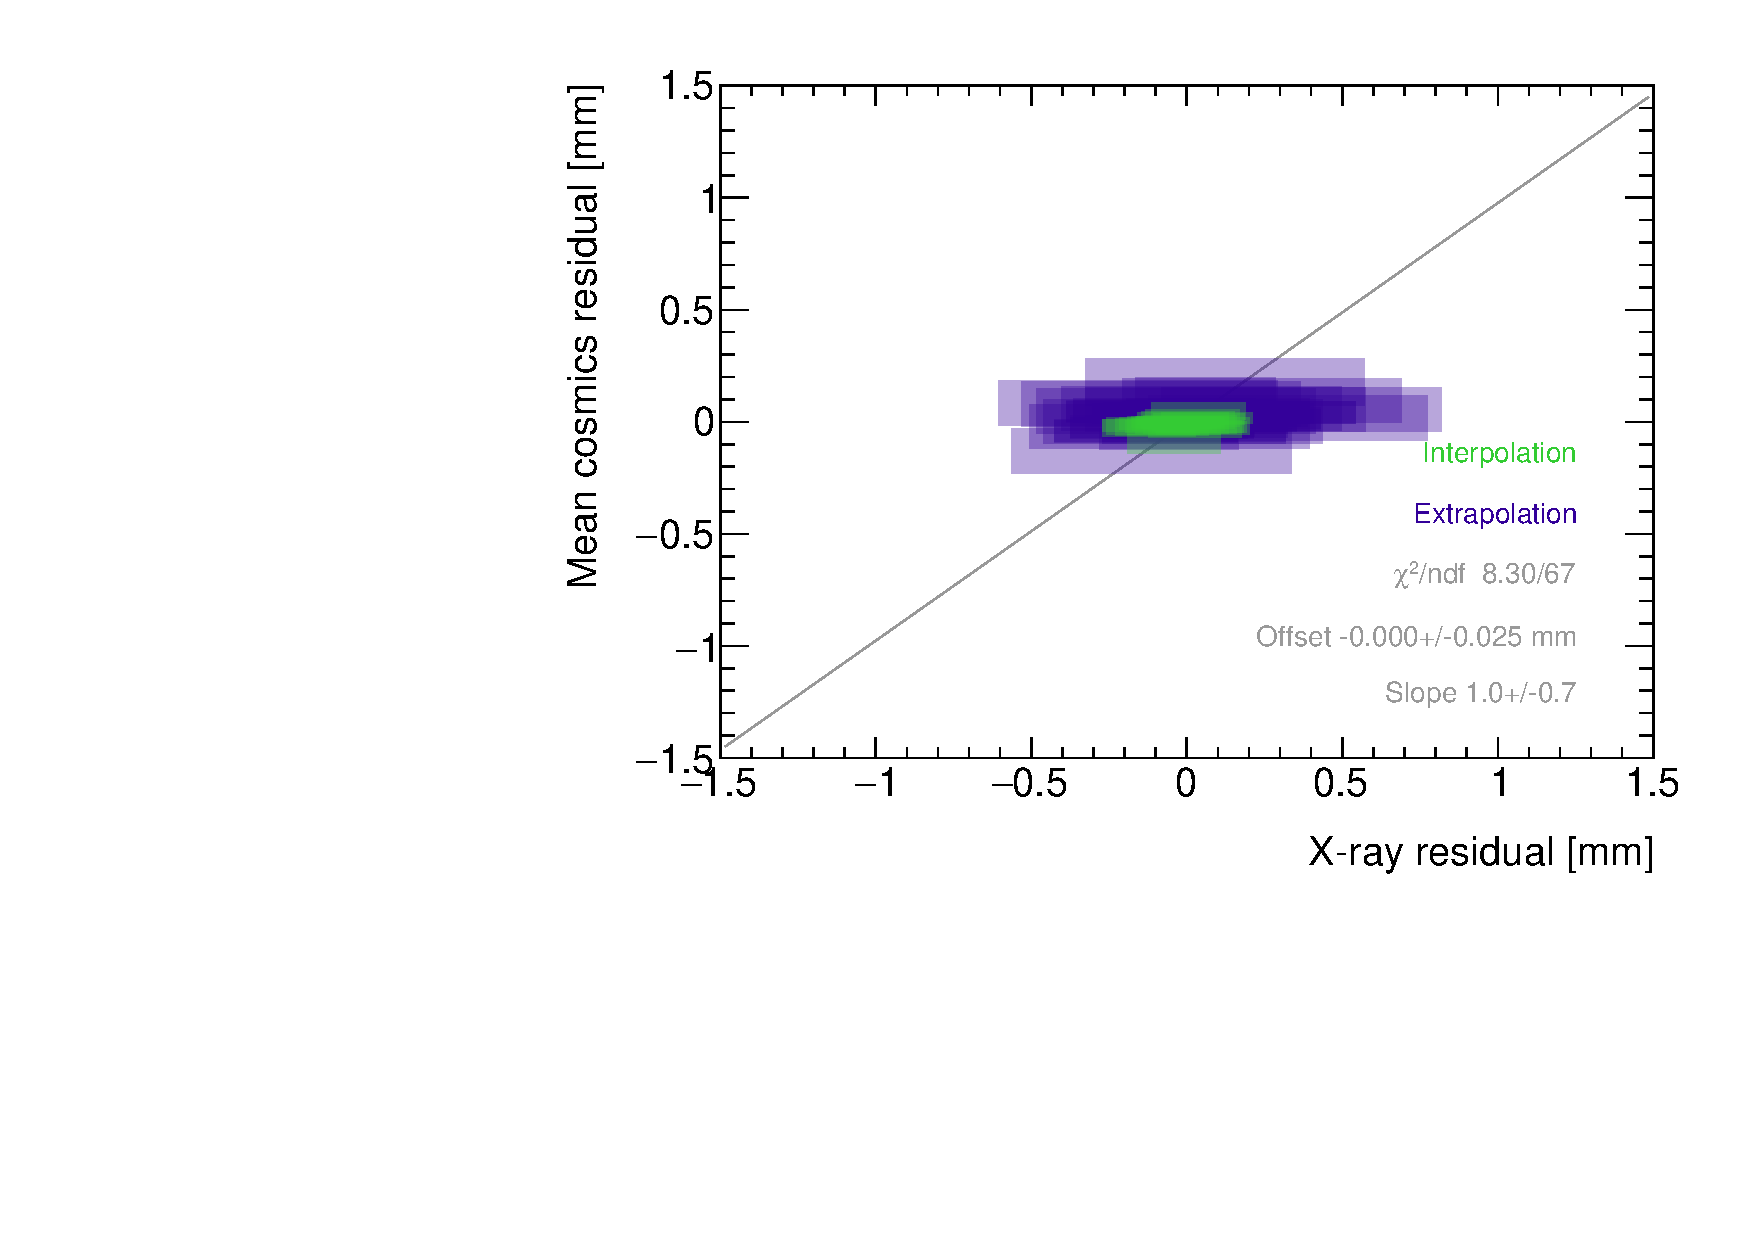
\includegraphics[width = \textwidth]{figures/figure_QL2P08_3100V_2021-08-16_QL2P08_local_cosmic_and_xray_data_correlation_plot.pdf}
    \caption{Correlation plot between x-ray and mean cosmics residuals for all tracking combinations for quadruplet 2. Each rectangle is centered on an x-ray and mean cosmics residual pair calculated at a given gun position and for a certain tracking combination. The width of the rectangles in $x$ and $y$ are the uncertainty in the x-ray and mean cosmics residual respectively. A printer-friendly version of this plot is available in appendix~\ref{appendix:print}.}
    \label{fig:no_correlation}
\end{figure}

Several quadruplets were tested for each quadruplet construction geometry built in Canada. Each quadruplet fell into one of the two categories: residuals large enough to see a correlation, or residuals too small to see a correlation. Since the x-ray and mean cosmics residuals were measures of the relative local offsets between the layer of a quadruplet and the two reference layers, quadruplets with the most relative misalignment had the largest range of residuals. the correlation plots were an easy visual way to identify quadruplets with large relative misalignments.

Residuals calculated with all tracking combinations are included in figures~\ref{fig:correlation} and \ref{fig:no_correlation}. There are three patterns in the residuals on the scatter plot explained by geometry. First, for both datasets the uncertainty in the extrapolated track residuals were larger than the interpolated track residuals because of the extrapolation lever arm. For the x-ray residuals, the effect of the lever arm on the uncertainty was direct since the residual was calculated from a single abstract track; for the mean cosmics residuals it was the widening of the residual distribution due to the extrapolation lever arm increasing the uncertainty in the fitted mean of residuals. Second, residuals calculated through extrapolation tend to be larger because the extrapolation lever arm can produce more extreme values of the track position on the layer of interest. Third, the points in figure~\ref{fig:correlation} are geometrically correlated (e.g. they seem to be roughly mirrored around the origin). This is expected since the residuals calculated using a given set of three layers should be geometrically correlated by the local offsets on the fixed layers and the layer of interest (the $d_{local, i}$ on each layer as defined in equation~\ref{eqn:local_translation}). 

% --------------------------------------------------
\section{Discussion}
% --------------------------------------------------
The most important limit on measuring the degree of correlation between the x-ray and cosmics residuals was the uncertainty on the x-ray residuals, which stemmed from the systematic uncertainty in the x-ray beam profile centers~\cite{lefebvre_precision_2020}. The method was limited primarily by the sTGCs' poor x-ray position resolution.

The analysis of certain quadruplets was also limited by the availability of data. Sometimes, less than three layers were surveyed for a given x-ray gun position so no residuals could be calculated. Too few x-ray residuals prevented the analysis from detecting a significant correlation, should it even be measurable. Often, the analysis of smaller quadruplets (placed innermost on the wheel) suffered as a result because they had fewer alignment platforms, and hence gun positions, on their surfaces. The analysis was also limited to certain quadruplets. The wedges constructed the earliest (typically small wedges) were surveyed when the method was still being designed and so have limited x-ray residuals calculated from beam profiles of lower quality. In addition, not all cosmic muon test sites had enough front end electronics to collect data on three layers simultaneously, which is the minimum required to be able to calculate residuals.

Nonetheless, the comparison of x-ray and cosmics residuals was really to confirm the x-ray method's ability to measure local offsets with an independent dataset. The x-ray absolute local offsets allow the calculation of relative local offsets that can be correlated to the cosmics relative local offsets. Therefore, the analysis of quadruplets with relative local offsets large enough to detect a correlation validates the x-ray method's ability to measure local offsets. The potential of using relative local offsets calculated from cosmics data to study relative alignment between sTGC layers stands on its own. It is especially compelling considering how much smaller the uncertainties in the relative local offsets are compared to the x-ray data.